\documentclass{article}
\usepackage[utf8]{inputenc}
\usepackage[
backend=biber,
style=alphabetic,
sorting=ynt
]{biblatex}
\addbibresource{cite.bib}
\usepackage{tikz}
\usepackage[left=1.8cm,right=1.8cm,top=2.2cm,bottom=2.0cm]{geometry}
\usetikzlibrary{shapes.geometric, arrows}

\newcommand{\code}[1]{\texttt{#1}}

\title{Proposal for CSE231 Course Project Multi-V-VM}

\date{October 2022}
\begin{document}
\author{\textbf{Yiwei Yang}~~\textbf{Pooneh Safayenikoo}~~\textbf{Zheyuan Chen}~~\textbf{Tongze Wang} \\ \texttt{ \{yyang363,psafyen,zchen406,twang141\}@ucsc.edu}}

\maketitle

\section{Introduction}
MVVM is a high-performance double JIT VM from RiscV assembly or elf to wasm, with all Linux implemented. Here 'V' can be translated into multiple meanings: RiscV, Variable Level, etc. The second from WASM VM can be run on the browser side since the WASM has already supported outer SDK for developers to insert other logic of optimization or security. We are proposing a comprehensive system emulator that implements the RISC-V privileged ISA and supports interrupts, memory-mapped input and output devices, a soft memory management unit with separate instruction and data TLBs, and other features.

\subsection{RiscV}
RiscV is the newly proposed reduced instruction set by UC Berkeley that was supposed to be a student course project, but it quickly be famous and widely used by multiple companies among countries as their main ISA for National Defence \cite{nasa} and unique configuration for commercial needs \cite{alibaba}. The decoding part for both RV32IMAFDV and RV64IMAFDV are different in instruction since the prior is 32bit length and with 32bit data, while the latter supports word(16bit), double word(32bit), and quadword(64bit) and the instruction are 64bit lengths. We need to implement them separately.

\subsection{WebAssembly}
WebAssembly is a new browser-supported feature that naturally supports the JIT at the ISA level. The browser has implemented a high-performance virtual machine called wasm3 \cite{wasm3} to support gaming \cite{senpai}, virtual machine \cite{windows2000} and video HVEC decoding\cite{bilibili}. Because of the non-SSA design of the ISA and easy to prove with isolation \cite{kwasm} and we've seen the application of isolation execution in serverless \cite{occlum} and blockchain smart contract with the booming of the increasingly secured and full-fledged compiler. 
\section{Insight and Novelty}
\begin{figure}[htbp]
\centering
   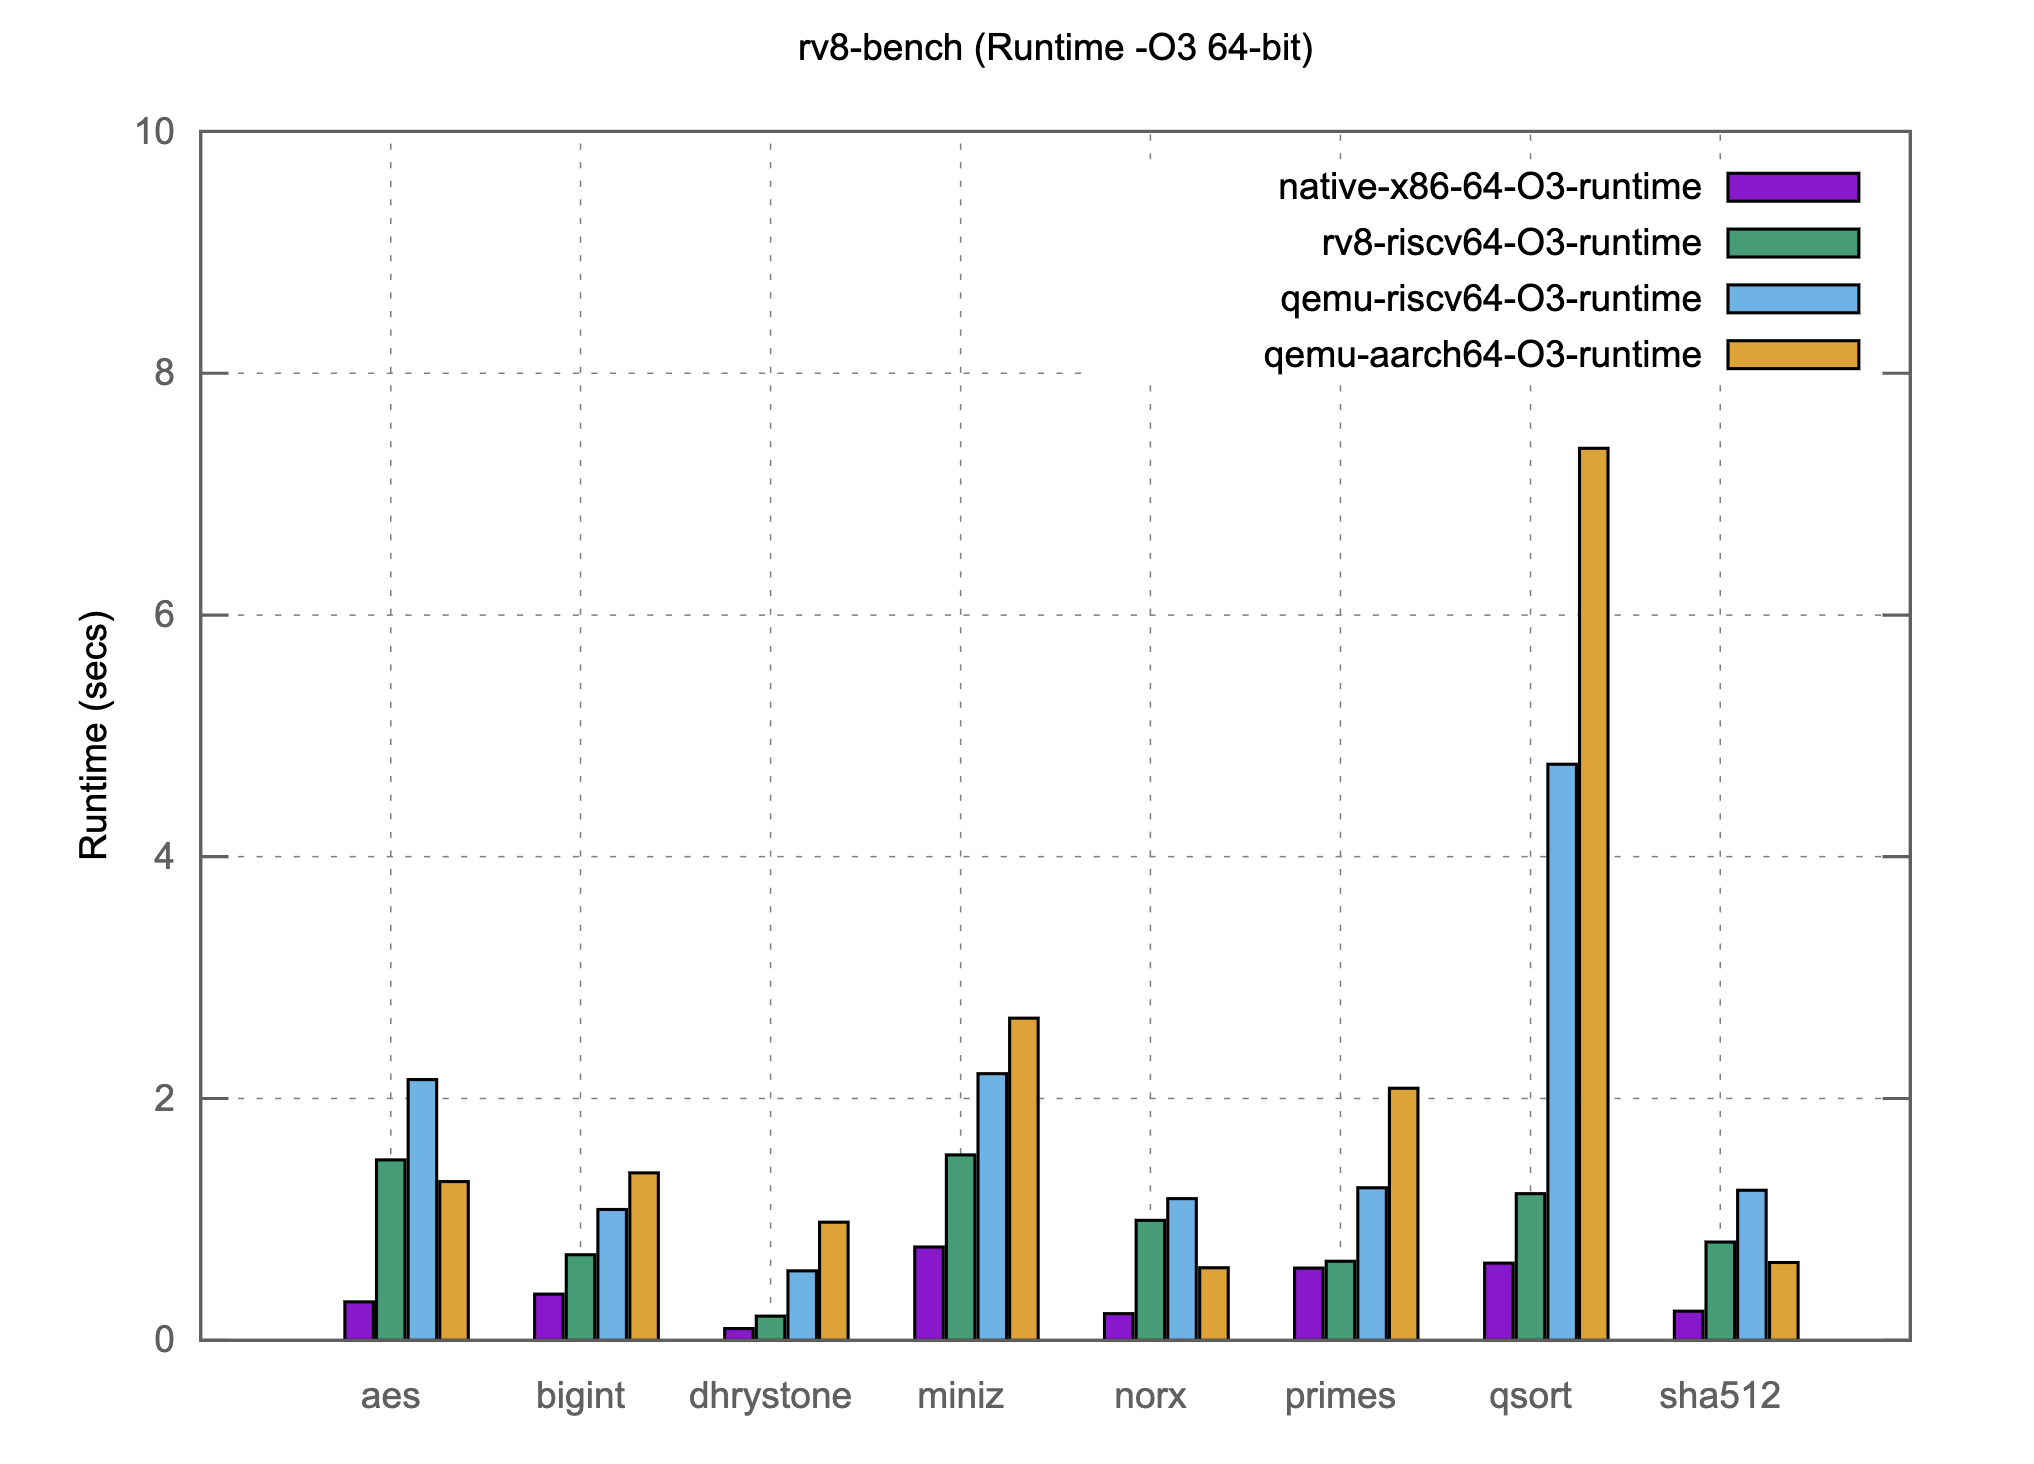
\includegraphics[width=0.4\textwidth]{rv8.png}
    \caption{JITed rv8 compared with JITed Qemu}
    \label{fig:my_label}
\end{figure}

We all know that we can simply apply the LLVM JIT with Qemu JIT to do the job, however, the transpilation speed is slow when you combine all the architecture. Since the abstraction of the assembly and the machine will not always be zero cost, you are always gonna save more abstracted types of instruction or runtime memory types which makes the JIT slow. As rv8 benchmark \cite{rv8} listed, we've already gained 10x speed up compared to Qemu. We support double layer JITed, in which the context of transpilation has both the information of the first layer and also can utilize the wasitime \cite{wasitime} JIT to optimize for the machine code.

\tikzset{every picture/.style={line width=0.75pt}} %set default line width to 0.75pt        
\begin{figure}[htbp]
\centering
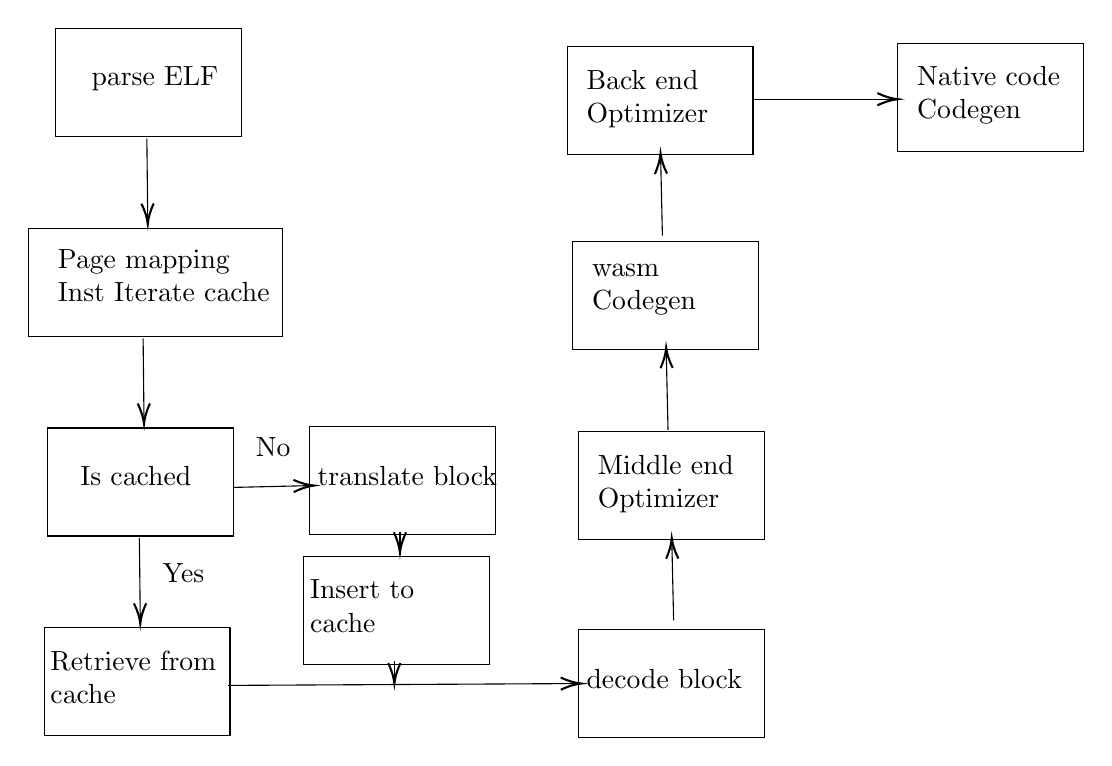
\begin{tikzpicture}[x=0.75pt,y=0.75pt,yscale=-0.9,xscale=0.9]
%uncomment if require: \path (0,657); %set diagram left start at 0, and has height of 657

%Shape: Rectangle [id:dp5630637521840367] 
\draw   (46,38) -- (145.5,38) -- (145.5,95.81) -- (46,95.81) -- cycle ;
%Straight Lines [id:da285430578197333] 
\draw    (95,97) -- (95.48,140.81) ;
\draw [shift={(95.5,142.81)}, rotate = 269.37] [color={rgb, 255:red, 0; green, 0; blue, 0 }  ][line width=0.75]    (10.93,-3.29) .. controls (6.95,-1.4) and (3.31,-0.3) .. (0,0) .. controls (3.31,0.3) and (6.95,1.4) .. (10.93,3.29)   ;
%Shape: Rectangle [id:dp2190977191270138] 
\draw   (31.5,145) -- (167.5,145) -- (167.5,202.81) -- (31.5,202.81) -- cycle ;
%Straight Lines [id:da0018857053885301678] 
\draw    (93,204) -- (93.48,247.81) ;
\draw [shift={(93.5,249.81)}, rotate = 269.37] [color={rgb, 255:red, 0; green, 0; blue, 0 }  ][line width=0.75]    (10.93,-3.29) .. controls (6.95,-1.4) and (3.31,-0.3) .. (0,0) .. controls (3.31,0.3) and (6.95,1.4) .. (10.93,3.29)   ;
%Shape: Rectangle [id:dp33637648003336396] 
\draw   (42,252) -- (141.5,252) -- (141.5,309.81) -- (42,309.81) -- cycle ;
%Straight Lines [id:da6058349373934426] 
\draw    (91,311) -- (91.48,354.81) ;
\draw [shift={(91.5,356.81)}, rotate = 269.37] [color={rgb, 255:red, 0; green, 0; blue, 0 }  ][line width=0.75]    (10.93,-3.29) .. controls (6.95,-1.4) and (3.31,-0.3) .. (0,0) .. controls (3.31,0.3) and (6.95,1.4) .. (10.93,3.29)   ;
%Straight Lines [id:da8091026554648684] 
\draw    (141.5,283.81) -- (182.5,282.86) ;
\draw [shift={(184.5,282.81)}, rotate = 178.67] [color={rgb, 255:red, 0; green, 0; blue, 0 }  ][line width=0.75]    (10.93,-3.29) .. controls (6.95,-1.4) and (3.31,-0.3) .. (0,0) .. controls (3.31,0.3) and (6.95,1.4) .. (10.93,3.29)   ;
%Shape: Rectangle [id:dp3506094282329688] 
\draw   (182,251) -- (281.5,251) -- (281.5,308.81) -- (182,308.81) -- cycle ;
%Shape: Rectangle [id:dp6135591324176446] 
\draw   (40,359) -- (139.5,359) -- (139.5,416.81) -- (40,416.81) -- cycle ;
%Straight Lines [id:da6922817779318298] 
\draw    (230.5,307.81) -- (230.5,316.81) ;
\draw [shift={(230.5,318.81)}, rotate = 270] [color={rgb, 255:red, 0; green, 0; blue, 0 }  ][line width=0.75]    (10.93,-3.29) .. controls (6.95,-1.4) and (3.31,-0.3) .. (0,0) .. controls (3.31,0.3) and (6.95,1.4) .. (10.93,3.29)   ;
%Shape: Rectangle [id:dp0944985393913289] 
\draw   (179,321) -- (278.5,321) -- (278.5,378.81) -- (179,378.81) -- cycle ;
%Straight Lines [id:da44984315062323565] 
\draw    (138.5,389.81) -- (325.5,388.82) ;
\draw [shift={(327.5,388.81)}, rotate = 179.7] [color={rgb, 255:red, 0; green, 0; blue, 0 }  ][line width=0.75]    (10.93,-3.29) .. controls (6.95,-1.4) and (3.31,-0.3) .. (0,0) .. controls (3.31,0.3) and (6.95,1.4) .. (10.93,3.29)   ;
%Straight Lines [id:da9404259452823103] 
\draw    (227.5,376.81) -- (227.5,386.81) ;
\draw [shift={(227.5,388.81)}, rotate = 270] [color={rgb, 255:red, 0; green, 0; blue, 0 }  ][line width=0.75]    (10.93,-3.29) .. controls (6.95,-1.4) and (3.31,-0.3) .. (0,0) .. controls (3.31,0.3) and (6.95,1.4) .. (10.93,3.29)   ;
%Shape: Rectangle [id:dp8711556627302299] 
\draw   (326,360) -- (425.5,360) -- (425.5,417.81) -- (326,417.81) -- cycle ;
%Shape: Rectangle [id:dp14704061025927073] 
\draw   (326,254) -- (425.5,254) -- (425.5,311.81) -- (326,311.81) -- cycle ;
%Straight Lines [id:da0676306392710595] 
\draw    (377,355) -- (376.05,313) ;
\draw [shift={(376,311)}, rotate = 88.7] [color={rgb, 255:red, 0; green, 0; blue, 0 }  ][line width=0.75]    (10.93,-3.29) .. controls (6.95,-1.4) and (3.31,-0.3) .. (0,0) .. controls (3.31,0.3) and (6.95,1.4) .. (10.93,3.29)   ;
%Shape: Rectangle [id:dp6677463790497207] 
\draw   (323,152) -- (422.5,152) -- (422.5,209.81) -- (323,209.81) -- cycle ;
%Straight Lines [id:da5451565013180288] 
\draw    (374,253) -- (373.05,211) ;
\draw [shift={(373,209)}, rotate = 88.7] [color={rgb, 255:red, 0; green, 0; blue, 0 }  ][line width=0.75]    (10.93,-3.29) .. controls (6.95,-1.4) and (3.31,-0.3) .. (0,0) .. controls (3.31,0.3) and (6.95,1.4) .. (10.93,3.29)   ;
%Shape: Rectangle [id:dp0342952207312206] 
\draw   (320,48) -- (419.5,48) -- (419.5,105.81) -- (320,105.81) -- cycle ;
%Straight Lines [id:da7090343492090339] 
\draw    (371,149) -- (370.05,107) ;
\draw [shift={(370,105)}, rotate = 88.7] [color={rgb, 255:red, 0; green, 0; blue, 0 }  ][line width=0.75]    (10.93,-3.29) .. controls (6.95,-1.4) and (3.31,-0.3) .. (0,0) .. controls (3.31,0.3) and (6.95,1.4) .. (10.93,3.29)   ;
%Shape: Rectangle [id:dp5561325788044003] 
\draw   (497,46) -- (596.5,46) -- (596.5,103.81) -- (497,103.81) -- cycle ;
%Straight Lines [id:da8172418973029782] 
\draw    (419,76) -- (495,76) ;
\draw [shift={(497,76)}, rotate = 180] [color={rgb, 255:red, 0; green, 0; blue, 0 }  ][line width=0.75]    (10.93,-3.29) .. controls (6.95,-1.4) and (3.31,-0.3) .. (0,0) .. controls (3.31,0.3) and (6.95,1.4) .. (10.93,3.29)   ;


% Text Node
\draw (64,57) node [anchor=north west][inner sep=0.75pt]   [align=left] {parse ELF};
% Text Node
\draw (46,155) node [anchor=north west][inner sep=0.75pt]   [align=left] {Page mapping\\Inst Iterate cache};
% Text Node
\draw (58,271) node [anchor=north west][inner sep=0.75pt]   [align=left] {Is cached};
% Text Node
\draw (102,323) node [anchor=north west][inner sep=0.75pt]   [align=left] {Yes};
% Text Node
\draw (152,256) node [anchor=north west][inner sep=0.75pt]   [align=left] {No};
% Text Node
\draw (185,271) node [anchor=north west][inner sep=0.75pt]   [align=left] {translate block};
% Text Node
\draw (42,370) node [anchor=north west][inner sep=0.75pt]   [align=left] {Retrieve from \\cache };
% Text Node
\draw (181,332) node [anchor=north west][inner sep=0.75pt]   [align=left] {Insert to \\cache };
% Text Node
\draw (329,380) node [anchor=north west][inner sep=0.75pt]   [align=left] {decode block};
% Text Node
\draw (335,265) node [anchor=north west][inner sep=0.75pt]   [align=left] {Middle end \\Optimizer};
% Text Node
\draw (332,163) node [anchor=north west][inner sep=0.75pt]   [align=left] {wasm\\Codegen};
% Text Node
\draw (329,59) node [anchor=north west][inner sep=0.75pt]   [align=left] {Back end \\Optimizer};
% Text Node
\draw (506,57) node [anchor=north west][inner sep=0.75pt]   [align=left] {Native code \\Codegen};


\end{tikzpicture}
    \caption{Diagram of the MVVM design doc}
\end{figure}
\subsection{Comparison between RiscV and WASM ISA}
\subsubsection{Code/Data Separation}
RiscV uses the same address space for code and data, while the running code of WASM does not even have a way to read/write itself. Simplify the implementation of the JIT compiler. If the code is self-modifying, then the JIT compiler needs to have the ability to detect changes and regenerate the target code, which requires a fairly complex implementation mechanism.
\subsubsection{Static types and control flow constraints}
WebAssembly is very "structural". The standard requires that all function calls, loops, jumps and value types follow specific structural constraints, e.g. passing two arguments to a function that takes three, jumping to a position in another function, performing a floating point add operation on two integers, etc. will result in compilation/validation failures; RISC-V has no such constraints, and the validity of instructions depends only on their own coding.
\subsubsection{Machine Model}
WebAssembly is a stack machine instruction set that will be JITed into the transpiled backend through a virtual machine, while RISC-V is a register machine instruction set.
\subsubsection{Memory Management}
Although WebAssembly and RISC-V both define an untyped, byte-addressable memory, there are some detailed differences between them; WebAssembly's memory is equivalent to a large array: the effective address starts at 0 and expands continuously up to some program-defined initial value and can grow. RISC-V, on the other hand, uses virtual memory, using page tables to map addresses to physical memory.
\subsubsection{Synchronization mechanism}
A Turing-complete calculator requires at least one conditional branch instruction. Similarly, an instruction set architecture that supports multi-threaded synchronization requires at least one "atomic conditional branch" instruction. Such instructions are available under WebAssembly and under RISC-V, corresponding to the CAS model and the LL/SC model, respectively. LL/SC has stronger semantics than CAS, which suffers from intractable ABA issues, but LL/SC does not. This also means that it is much more difficult to simulate LL/SC on a CAS architecture than vice versa.

\section{Proposed Architecture}
\subsection{Front end}
We first parse the RiscV assembly. By getting the metadata in the elf, we know the linkage type, which architecture and etc. We then do the memory mapping to the WASM, during which we parse the instruction one by one using rust iterator and decoding using a code cache so that it will cache the block that has been translated before for better frontend optimization.
\subsubsection{Normal Instruction}
31 general-purpose registers and 31 floating point general-purpose registers(both have hard-wired zero) will be compiled completely to the WASM memory stack machine which we'll be LRU for register-stack mapping. As for function calls and the semantics of the stack frame and local variable, we will just translate how WASM interacts with the call convention.
\subsubsection{RVV Instruction}
We are supposed to support RVV Instructions, which add the \code{VLEN} global environment for one core. WASM has already equipped with basic SIMD \cite{wasm-simd}, which is just a mapping of SSE2. So the question is mapped to transpile from one SIMD to the other implementation of SIMD.
\subsubsection{Multi Process Support}
We will fully emulate how the process's order of accessing the variable to the semantic level. Since the semantic of RVWMO, the emulation of the weaker memory model will automatically be done on the stronger memory model, all we need to take care of is intrinsic of load\_seq and store\_release of taking care of atomic variable, which we can assign those to the atomic variable of a variable. Since the analysis through a wider range of searches for those atomic variables is hard, we try to map the semantics of RV as strong or conventional as possible.
\subsubsection{Privilege Instruction}
For different rings inside RiscV, we have to follow the semantics of the guest address and host address translation and we have to provide a software MMU here to get the translation right. In WASM, we think the same process shares nothing by addresses, thus the MMU for WASM is unnecessary.
\subsection{Middle end}
During translating the instruction, we have a middle end for optimizing from RiscV to WASM like the Solid-State Register Allocator \cite{ssrc}.
\subsection{Back end}
We need a WASM Runtime for LibC in the first place. Although there already exists a WASI implementation \cite{wasi-sdk}, we think we just need a lightweight Runtime for a better performance
\subsubsection{LibC}
There are 2 major Libc implementations out there, we are choosing \code{musl} for its simplicity. Let's give a comparison between \code{musl} and \code{sysv}. \cite{musl-sysv-compare}
\begin{enumerate}
    \item \code{musl} is a much simple standard library compared to GlibC. When linked statically, binary files will be more size-efficient 
    \item \code{sysv} has more depth to get to call the real syscall stub, which is more heavy weighted.
\end{enumerate}
\subsubsection{Optimization}
We can cast optimization over the wasitime-jit since they provide a context for code generation. We can have the following prospective optimization from WASM to native code.
\begin{enumerate}
\item Function Inlining
\item Common Expression Elimination
\end{enumerate}
\section{Conclusion}
In the final report, we will provide a systematic review of different implementations of different RiscV VM from functionality and performance. 
\printbibliography
\end{document}
